%
% 
%
\let\textcircled=\pgftextcircled
\chapter{Experimental Methods}
\label{chap:expMethods}

\initial{I}n this chapter we introduce general methods for the synthesis, imaging, and analysis of colloidal particles. We begin with an introduction to laser scanning confocal microscopy; which is the technique used in later results chapters to image colloidal particles in real-time. We then detail the synthesis protocols for the creation of the fluorescent colloids that are used to form the gel network, as well as detailing the process for the creation of Janus particles. We then finish with an introduction to the particle analysis methodologies used in this work: particle tracking and the chord length distribution.




\section{Laser scanning confocal microscopy}
Colloids possess a lengthscale on the order of visible light and so are amenable to optical microscopy techniques. However, this size has an additional effect in that for dense suspensions, the colloids cause a large degree of light scattering leading to poor image quality. This effect can be reduced with a combination of two factors: the imaging of only one single point of the sample at a time, and the addition of a pinhole before the detector. The former acts to reduce scattered light from outside the region of interest, while the pinhole rejects light from outside of the focal plane. These are the principles of confocal microscopy, and with these in place the single point is scanned across the focal plane to produce a 2D image. This image comprises one single plane in the sample, and through systematic altering of the focal plane, a 3D image can be constructed from a stack of 2D scanned images. Image quality is further improved with a laser light source, providing greater point illumination \cite{paddock1999}. This system can be further specialised for the observation of fluorescent samples, where multiple excitation wavelengths can be selected for, allowing for multiple species to be imaged independently. The light from the resultant emission is then passed through a filter before entering the lens, and thus all light from the laser illumination is discarded from the final image \cite{paddock1999}. For these reasons, laser scanning confocal microscopy is the ideal solution for high-resolution  imaging of 3D colloidal systems.



\section{Particle synthesis}
\label{sec:particle_synthesis}

In the experimental system we require two species of particle: plain silica particles and Janus particles. The silica particles will form the colloidal gel, while the Janus particles undergo active dynamics. The two particle species must be distinguishable during experimental observation, and therefore we use two fluorescent dyes with distinct emission spectra: rodamine for the gel and fluorescein for the Janus particles. 
The two dyes differ in their excitation ($\lambda_{\textrm{ex}}$) and emission ($\lambda_{\textrm{em}}$) wavelengths. For rodamine $\lambda_{\textrm{ex}} = 546$nm and $\lambda_{\textrm{em}} = 568$nm, while for fluorescein $\lambda_{\textrm{ex}} = 498$nm and $\lambda_{\textrm{em}} = 515$nm.
For the plain silica, we synthesise particles with a core-shell structure, where the core contains the fluorescent dye and is surrounded by a shell of undyed silica. This greatly improves the resolution during microscopy as it acts to separate the particle centres. This is especially useful in dense regions (such as the branches of a colloidal gel).
In this section we detail the methods for the creation of both the core-shell silica particles and the Janus particles.


\subsection{Synthesis of fluorescent silica nanoparticle cores}

\textit{Synthesis of nanoparticle cores ---} the colloidal silica nanoparticles created for this work are synthesised through a hydrolysis-condensation reaction known as the St\"{o}ber process \cite{stober1968}. This chemical process is a widely used method for the synthesis of silica nanoparticles, and is ubiquitous in colloidal science as a result of the low polydispersity of the resultant particle sizes. The reaction is carried out in a one-step process within a single reaction vessel, where both hydrolysis and condensation reactions happen simultaneously \cite{vanblaaderen1992,chen1996}. The reaction occurs as follows: 
	The silica precursor tetraethyl orthosilicate (TEOS) ($\mathrm{Si}(\mathrm{OC}_2\mathrm{H}_5)_{4}$) undergoes a hydrolysis reaction in ethanol ($\mathrm{C}_2 \mathrm{H}_5\mathrm{OH}$) catalysed by ammonium hydroxide (NH$_3$):

\begin{equation}
	\mathrm{Si}(\mathrm{OC}_2\mathrm{H}_5)_{4}+4 \mathrm{H}_{2} \mathrm{O} \rightarrow \mathrm{Si}(\mathrm{OH})_{4}+4\mathrm{C}_2 \mathrm{H}_5\mathrm{OH}
\end{equation}


\noindent This reaction produces ethoxysilanol ($\mathrm{Si}(\mathrm{OH})_{4}$) and ethanol. These ethoxysilanols can then undergo a condensation reaction with another silanol or TEOS to produce silica:


\begin{equation}
	n\mathrm{Si}(\mathrm{OH})_{4} \rightarrow n\mathrm{SiO}_{2}+2n\mathrm{H}_{2} \mathrm{O},
\end{equation}

\noindent where $n$ is an integer. The continuing cycles of hydrolysis and condensation result in the cross-linking and gradual formation of the silica particles. For the generation of 440nm diameter cores we follow the recipe of Rossi \etal \cite{rossi2005}.



\textit{Incorporation of the fluorescent dye ---} for the production of fluorescent silica particles we follow the methodology of van Blaaderen \etal \cite{vanblaaderen1992}, where nanoparticle cores are grown in the presence of a fluorescent dye (rodamine). To incorporate the dye throughout the entirety of the particle, the dye must be linked to a silane coupling agent (3-aminopropyl)triethoxysilane (APS). This process makes use of the amino group of APS and the thioisocyanate group of rodamine to perform an addition reaction, forming a covalent bond. In this form, the rodamine can be incorporated into the silica during the cross-linking of ethoxysilanols.

\subsection{Synthesis of core-shell silica nanoparticles}
\label{sec:core_shell}

\begin{figure*}
	\centering
	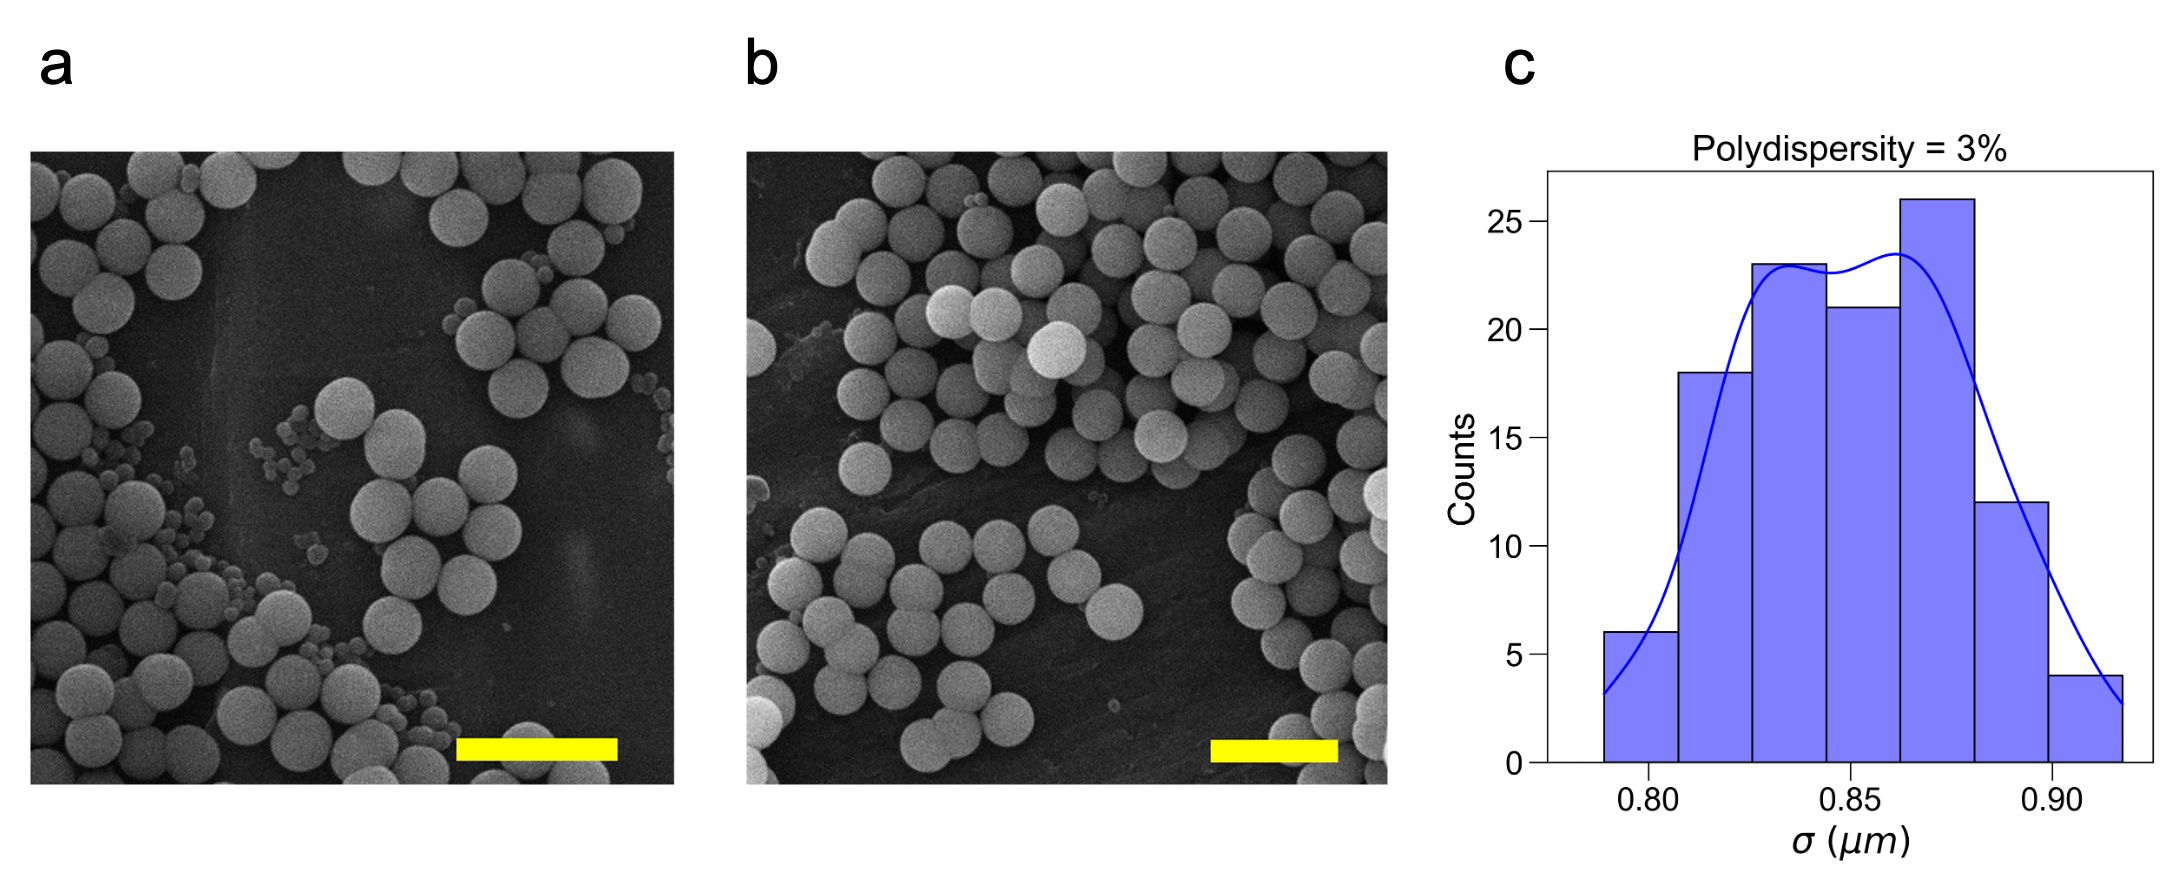
\includegraphics[width=\linewidth]{figsExpMethods/figParticleSize}
	\caption[Synthesis of silica nanoparticles]{Scanning electron microscopy images of silica particles: \textbf{a} An example of secondary nucleation. Small particles have been created during the shell growth and can be seen in between the larger dyed particles. Scale bar $2\mu$m. \textbf{b} An example of a successful shell growth reaction. The particles have grown from $\sim$440nm diameter cores to around 850nm in diameter. There are some signs of secondary nucleation but it has been kept to an acceptable level. Scale bar $2\mu$m. \textbf{c} the particle size distribution for the particles depicted in b and used to form the colloidal gel.}
	\label{fig:sem}
\end{figure*}


Once the fluorescent silica cores have been prepared, a second growth process is carried out to produce the non-dyed shell layer. For this process, one needs to take great care that any new silica growth happens on the surface of the existing cores, and not as nucleation of secondary particles. 
For the shell growth, we suspend silica cores in ethanol and ammonium hydroxide as before, and to this a calculated concentration of TEOS is added. To determine the quantity of TEOS required to grow cores of a starting diameter $\sigma_{s}$ up to a final diameter $\sigma_{f}$. Following Chen \etal \cite{chen1996}, we use the relation:

\begin{equation}
	\left( \frac{\sigma_{f}}{\sigma_{s}}\right)^{3} = \frac{W_{c} + W}{W_{c}}
\end{equation}

\noindent where $W_{c}$ is the weight present as cores, and $W$ is the weight of silica added in the form of TEOS.
To avoid secondary nucleation, the ratio between the rate of consumption (use of TEOS for shell growth) and the rate of regeneration (use of TEOS in nucleation of new cores) must be controlled. For shell growth, the generation rate must be lowered \cite{chou2008,bogush1988}, an example of secondary nucleation is shown in Fig. \ref{fig:sem}a. This can be avoided by adding the desired quantity of TEOS in small batches throughout the process, and thus keeping the concentration of TEOS low during the reaction. For the particles in this work, a shell was grown on to the 440nm cores such that the new diameters approximately 850nm. This was achieved with the Stöber process following Graf \etal \cite{graf2003} with a TEOS concentration of [0.2M] added in six batches at one hour intervals. This process was repeated twice more to reach the desired diameter. These particles were imaged with scanning electron microscopy and an example is shown in Fig. \ref{fig:sem}b. The average particle diameter was determined through analysis of these images, the results are plotted in Fig. \ref{fig:sem}c, where the mean value is 850nm. For colloidal particles, the size distribution is often characterised by the polydispersity, defined as the ratio between the mean and the standard deviation: $s = \sqrt{\langle \sigma^2 \rangle - \langle \sigma \rangle^2}/\langle \sigma \rangle$. $s$ was measured to be 3\% for these particles.



\subsection{Synthesis of Janus particles}
\label{sec:janus}
The metallodielectric Janus particles used in this work are comprised of a silica core, upon which a thin layer of chromium is masked on to one hemisphere. The response of Janus particles to electric fields is dependant on the particle size \cite{gangwal2008}. The particles synthesised via the methods outlined above are too small and so silica cores of diameter 1.5$\mu$m were purchased (Kisker Biotech). These particles have a very low polydispersity and are dyed with fluorescein.

For the metallic coating, the silica particles are suspended in isopropanol at a low colloid volume fraction: $\phi_c = 0.075$. This suspension is then deposited and spread on to glass microscopy slides to form a monolayer as the solvent evaporates \cite{jeong2010}. The function of the monolayer is such that metal deposited from above can only reach one hemisphere, and all particles are equally exposed. The metal layer is deposited with e-beam lithography to a thickness of 3nm. Following this a 30nm layer of silica is added on top of the metal (also with e-beam), to screen strong charge interactions between particles, that would result from the exposed metal surface.
 



\section{Particle tracking}
\label{section:expMethods:ParticleTracking}
One key advantage of confocal microscopy over many other techniques is the ability to image systems in 3D dimensions. From this data, it is possible to apply image analysis techniques to extract the individual particle coordinates from a stack of 2D slices. For the extraction of coordinates from these 3D images, the particles in a slice are considered not only in that specific slice but in the context of slices above and below. For tracking of dense 3D images a combination of two tools are used: \textit{trackpy v0.5.0} \cite{allan2021}, and \textit{nplocate} \cite{yang2022}. The former is based on an implementation of the Crocker-Grier algorithm \cite{crocker1996} and the later uses the result from trackpy to simulate an image, and making adjustments by adding particles and displacing particles to converge towards the original input image. 

For 2D microscopy data where the sample is relatively dilute, it is quicker and more accurate to manually track the particles using \textit{Fiji} \cite{schindelin2012}. The image data extracted from confocal microscopy contains spacial information and so one can manually select and measure the particle positions directly from the image.


\section{Chord length}

\begin{figure*}
	\centering
	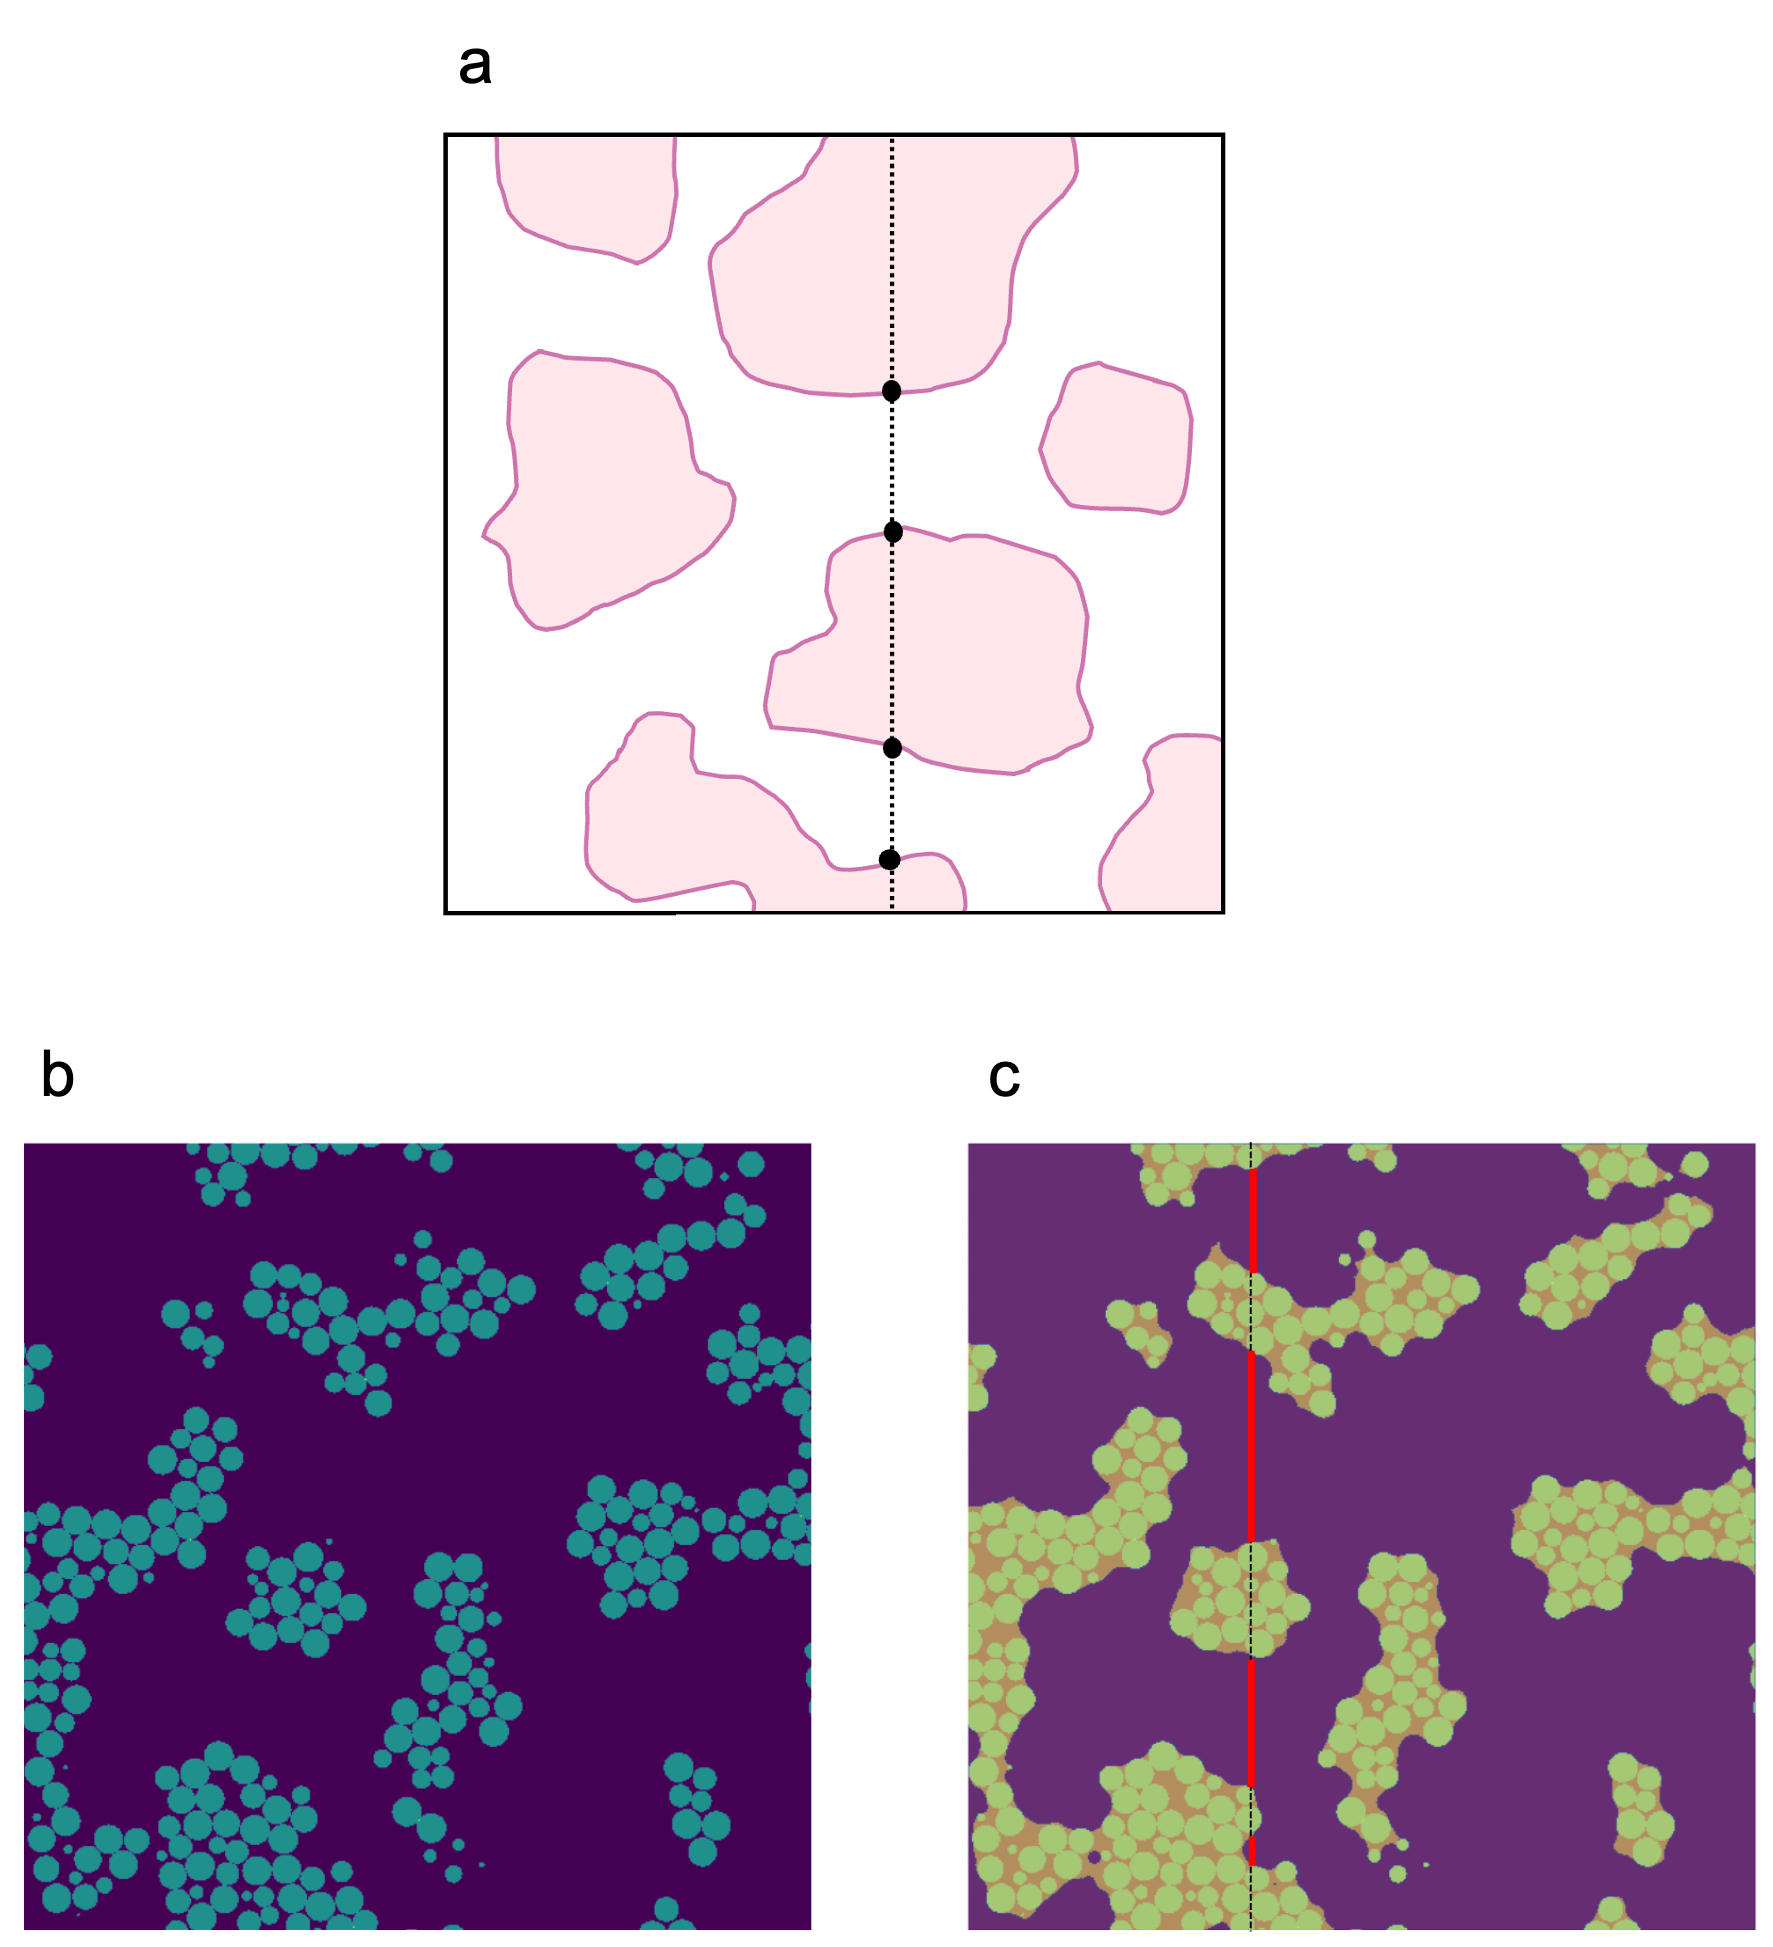
\includegraphics[width=0.8\linewidth]{figsExpMethods/figChordLength.png}
	\caption[Determination of the chord length in heterogeneous systems]{The chord length in heterogeneous systems. \textbf{a} Schematic of chord length measurements of a two-phase random material. Chords are defined by the interaction of lines with the two phase media. \textbf{b} An example of a 3D gel converted into a binary pixilated image. We show a slice through the 3D system where the gel phase is shown in blue and the pore phase is shown in purple. \textbf{c} Following the dilation/erosion process the pore chord lengths are measured. Yellow areas show original particle material, orange areas show the internal area. Yellow and orange areas are considered equal. Red lines show example chords in the pore phase.}
	\label{fig:methods:ChordLength}
\end{figure*}

 Across a wide variety of systems, the structure and lengthscales of porous networks have profound effects on the transport properties of any fluid or material within \cite{torquato1991,hofling2013}. The complex environments used in this work are heterogeneous systems: the self-assembly of a colloidal gel leads to the appearance of a porous network surrounding the particle aggregates; and randomly pinned spheres create a complex porous structure in the space surrounding them. To characterise the lengthscales of these porous systems we measure the chord length distribution \cite{torquato}. A chord is defined as the distance between two interfaces in a heterogeneous system, where the chord lies wholly within one phase (Fig. \ref{fig:methods:ChordLength}a). The chord length distribution function $p(\ell)$, defines the probability of finding a chord of length between $\ell$ and $\ell + d\ell$ within one phase. 
 
 In practise, chords are measured independently along each dimension of a lattice used to coarse grain the density \cite{testard2011}. This can be calculated for an experimental system where the particle coordinates have been determined with particle tracking. Assuming mono-disperse spheres, these coordinates are reconstructed in a 3D binary image, where particles have a diameter of 20 pixels. An example is shown for a model gel in Fig. \ref{fig:methods:ChordLength}b, where a slice is taken through the 3D system: blue regions correspond to the colloid phase and purple regions correspond to the pore phase. This image could be used to measure the chord distribution, however for the purpose of measuring the lengthscales relevant to active particles within the pores, the small chords within the colloid branches ought to be removed. This is because due to the excluded volume interactions, the interior of the gel branches are inaccessible to the active particles. Moreover, due to the packing of spheres these regions are interspersed with narrow channels of the pore phase which will bias the measurement of chords to low values. Therefore, we perform a sequential dilation-erosion process such that these small gaps are filled, the result of which is shown in Fig. \ref{fig:methods:ChordLength}c. Here we have overlayed the original image with the modified version. Yellow and orange regions are considered one phase and define the inaccessible volume. The surrounding purple phase is the porous network and is the phase upon which the chords are measured. In Fig. \ref{fig:methods:ChordLength}c we highlight an example of chords measured in one dimension (red).
 This is a versatile method and functions for any system of spherical particles. As well as analysis of experimental colloidal gels, we perform this analysis for simulated systems of model gels and randomly pinned spheres. 
 
 %Further technical details are provided in the \fergus{supplementary information.}

 
 
 %\section{Preparing samples at a known volume fraction}

%\fergus{
%
%\begin{equation}
%	\phi_c = \frac{V_c}{V_{\textrm{Total}}} = \frac{0.64\rho_c m_{\textrm{sd}}}{m_{\textrm{sd}}(0.64\rho_c  + 0.36\rho_{\textrm{s}}) + V_{\textrm{s}}}
%\end{equation}
%
%Here, $V_c$ is the volume of colloids in the sample, $V_{\textrm{Total}}$ is the total sample volume, $\rho_c$ and $\rho_s$ are the densities of the colloids and the solvent respectively, $m_{sd}$ is the mass of the sediment, and $V_s$ is the volume of solvent added to the sediment to reach the desired volume fraction.}
%
%\fergus{
%		\begin{equation}
%			\phi_p = \frac{V_p}{V_\textrm{Total}} = 
%		\end{equation}
%		}


%In chapter \ref{chap:colloids}, we explained the importance of the volume fraction as a control parameter for both hard spheres and colloid-polymer mixtures. It is therefore essential that we are able to control this parameter in experiment.

%\textit{Colloid volume fraction ---} 
%here the volume fraction describes the fraction of the total system volume occupied by colloids, a there are multiple methods for preparing samples with the appropriate proportions. In this work, the colloids are stored in solvent and so the method must acknowledge the presence of the solvent when samples are measured. 
% to prepare a suspension of silica colloids at a desired volume fraction, colloids are suspended in solvent and centrifuged. This forces the colloids to form a solid in the container, above which the majority of the solvent sits as a supernatant. If the supernatant is removed, the remaining sample is comprised of colloids at a volume fraction of $\phi_c = 0.64$ in solvent. This is based on the assumption that colloids are hard spheres and have formed a solid at random close packing. Therefore, if this sediment is weighed ($m_{\mathrm{sediment}}$), the volume of silica $V_{\mathrm{silica}}$ can be determined using the known density of silica $\rho_{\mathrm{silica}}=2$g/cm$^3$ and the assumption of random close packing: $V_{\mathrm{silica}} = 0.64(m_{\mathrm{sediment}}/\rho_{\mathrm{silica}})$. This sediment can then be diluted with a specific volume of additional solvent such that the sample is at the desired volume fraction:
% 
% \begin{equation}
% 	V_{\mathrm{solvent}} = \frac{V_{\mathrm{silica}} - (\rho_{\mathrm{desired}} )}{}
% \end{equation}
%
%\textit{Polymer volume fraction ---}


